\documentclass[11pt,a4paper]{article}
\usepackage[utf8x]{inputenc}
\usepackage[spanish]{babel}
\usepackage{amsmath}
\usepackage{graphicx}

\title{My Personal Newton}
\author{Juanma Cruz \\ juacrumar@gmail.com}

\begin{document}

\maketitle

\section{Nombre}
Git... Nuevo Repositorio... ¿Vaya? ¿Nombre? Nombre, nombre, nombre, nombre. Nombre. No. Muy malo. A ver, vamos a hacer cosas relacionadas con la gravedad... ¡Graviteitor! No. Muy malo. A ver, piensa... ¡Oh! ¡Newtoneitor! ¡Todo el mundo relaciona Newton con la gravedad!

\section{Cáculo de la gravedad}
Este documento no pretende ser un manual de física básica (de eso hay algunos muy buenos) sino simplemente una explicación breve de lo que hace el programa y cómo lo hace.

\begin{equation}
g = G\frac{M}{r^2}
\end{equation}

Hasta aquí la fórmula típica para calcular la aceleración que un cuerpo de masa $M$ ejerce en un punto determinado del espacio a una distancia $r$. En todo momento estoy tomando a los planetas como esferas perfectas (esto es, como un punto que tiene toda la masa, viajando por la órbita del planeta).

Para la gravedad que ejerce la tierra he hecho un poco de trampa y he tomado como base el famoso $g_0 = 9.8 m/s^2$, haciendo la diferencia respecto al nivel del mar como un simple coeficiente. Si $R$ es el radio de la Tierra y $h$ la altura sobre el nivel del mar.

\begin{equation}
    g(h) = g_0\left(\frac{R}{R+h}\right)^2
\end{equation}

\section{Cálculos de órbitas}
Para el cálculo de la distancia entre el usuario y el planeta en cuestión me he tomado la libertad de realizar una serie de aproximaciones:

\begin{itemize}
    \item La Tierra es un punto en el espacio. Esta aproximación solamente tiene algún efecto en el caso de la luna\footnote{Y no es un efecto importante, aunque es un plan de futuro tener en cuenta el radio de la tierra}
    \item En esta primera versión, las órbitas coexisten todas en el mismo plano y son perfectamente circulares, aunque pretendo programarlas como elipses en el futuro (no, no es complicado, pero como prueba de concepto quería tener también el circular y empecé por ahí). Esta aproximación es realmente buena en todos los casos que no son Plutón.
\end{itemize}

\begin{figure}{h}
    \centering
    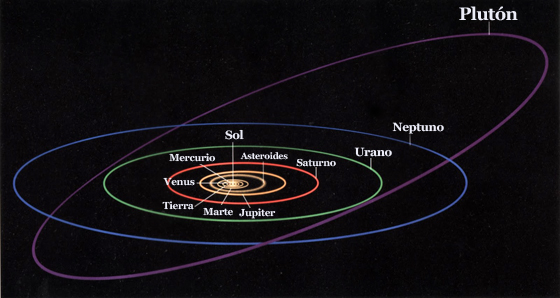
\includegraphics[width=0.5\textwidth]{orbitas.png}
    \caption{Have you heard about Pluto? That's messed up, right?}
\end{figure}

\end{document}
